% Provenance (never printed): see sources/outline_sources.md and sources/book1/BRIEFS.md (g6/03).
% Drawings: code/grade-6/03-for-loops-turtle/figures/record_turtle.py writes figures/out/*.dat from the
% unchanged listings (code/shared/turtlerec). Rerun it after changing a turtle listing.
\chapter{Repeating with \texttt{for}: Turtle Drawings}\label{ch:g6:for-loops-turtle}

Leo has written a \omterm{def:g4:programs-and-operating-system:program}{program} that draws a square: two lines, ``go forward'' and
``turn left'', written four times. Now he wants a shape with 36 sides, almost a
circle. That would be 72 lines, all the same, and one typing mistake would spoil
the shape. There must be a better way: a \omterm{def:g1:what-is-a-computer:computer}{computer} is very good at doing the same
thing again and again, if we tell it how many times.

\begin{recall}
An \omterm{def:g4:algorithms-repeat-and-decide:algorithm}{algorithm} can say ``repeat 4 times'' instead of writing the same steps four
times (\cref{ch:g4:algorithms-repeat-and-decide}). A \omterm{def:g6:variables-and-input:value}{variable} is a name for a
\omterm{def:g6:variables-and-input:value}{value}, and an \omterm{def:g6:variables-and-input:assignment}{assignment} such as \code{n = 6} gives it a \omterm{def:g6:variables-and-input:value}{value}
(\cref{ch:g6:variables-and-input}).
\end{recall}

\section{The turtle}

\begin{definition}[Turtle graphics]\label{def:g6:for-loops-turtle:turtle}
\emph{Turtle graphics}\index{turtle graphics} is a way of drawing with a
\omterm{def:g4:programs-and-operating-system:program}{program}: a pen, called the turtle, moves on the screen and leaves a line behind
it. It has a position and a heading, the direction it faces, and it obeys
\code{forward(d)} (move $d$ steps straight ahead), \code{left(a)} and
\code{right(a)} (turn on the spot by $a$ degrees), \code{penup()} and
\code{pendown()} (lift or lower the pen).
\end{definition}

The turtle starts in the middle of the window, facing right. Python's
\code{turtle} module brings these \omterm{def:g1:instructions-in-order:instruction}{instructions}; a \omterm{def:g4:programs-and-operating-system:program}{program} first takes the ones
it needs with \code{from turtle import ...}. Its last line, \code{done()}, keeps
the window open until it is closed.

\begin{omfigure}
\begin{tikzpicture}[x=1cm, y=1cm, font=\footnotesize,
    turt/.style={fill=ocMint!70!black, draw=black!70}]
  \draw[black!15, step=1] (-0.5,-0.5) grid (3.5,2.5);
  \fill[turt] (0,0) ++(0.32,0) -- ++(-0.5,0.2) -- ++(0,-0.4) -- cycle;
  \draw[-{Stealth[length=2mm]}, ocRed, thick] (0,0) -- (0.9,0);
  \node[below] at (0,-0.5) {start: at $(0, 0)$, facing right};
  \begin{scope}[shift={(6,0)}]
  \draw[black!15, step=1] (-0.5,-0.5) grid (3.5,2.5);
  \draw[very thick] (0,0) -- (2.5,0);
  \fill[turt] (2.5,0) ++(0,0.32) -- ++(0.2,-0.5) -- ++(-0.4,0) -- cycle;
  \draw[-{Stealth[length=2mm]}, ocRed, thick] (2.5,0) -- (2.5,0.9);
  \draw[->, black!60] (2.95,0) arc[start angle=0, end angle=90, radius=0.45];
  \node[right, black!60] at (3.0,0.35) {$90^\circ$};
  \node[below] at (1.25,-0.5) {after \code{forward(50)} and \code{left(90)}};
  \end{scope}
  \draw[-{Stealth[length=2.5mm]}, thick, black!60] (3.9,1) -- (5.3,1);
\end{tikzpicture}

{\small The turtle's state is its position and its heading (the red arrow).
\code{forward} changes the position and draws; \code{left} changes only the
heading.}
\end{omfigure}

\omcode{code/grade-6/03-for-loops-turtle/listings/square_long.py}{1}{11}{A square,
the long way.}\label{lst:g6:for-loops-turtle:square-long}

When the \omterm{def:g4:programs-and-operating-system:program}{program} runs, a window opens and the turtle draws a square of side
100. In this book, the turtle drawings are printed from the turtle's recorded
path rather than as a picture of the window.

\begin{history}[A turtle on the floor]
% ledger: g6:logo-1967, g6:logo-floor-turtle, g6:valiant-turtle
The turtle comes from Logo, a \omterm{def:g6:first-python-program:language}{programming language} for children created in
1967 by a team led by Wallace Feurzeig, with Seymour Papert and Cynthia Solomon.
The first turtle was a small robot on the floor, carrying a pen and drawing on
large sheets of paper; it soon moved to the screen. Floor turtles were still
sold to schools in the 1980s.

\medskip
\begin{center}
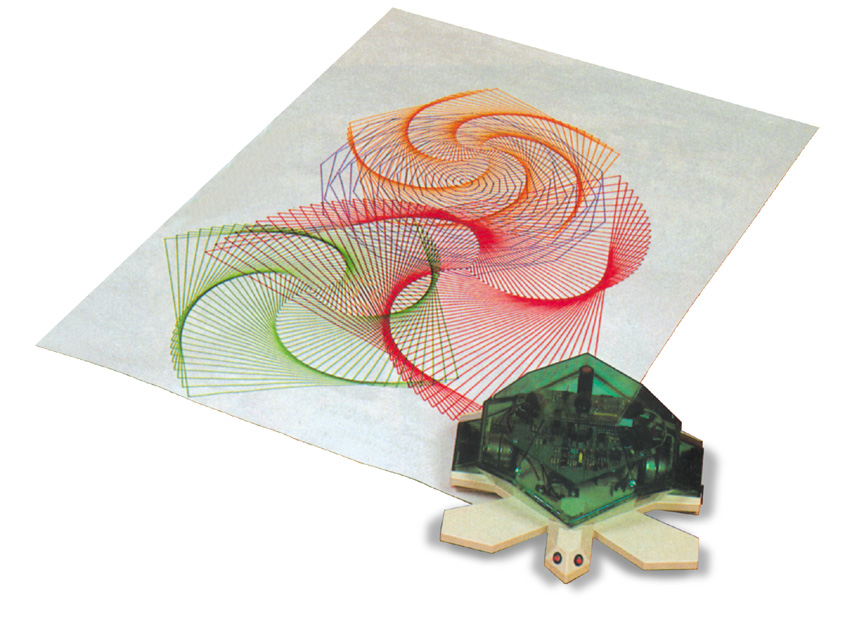
\includegraphics[width=0.5\linewidth]{images/book1/g6-valiant-turtle.jpg}

{\small A floor turtle robot of the 1980s, with a drawing it made.}
\end{center}
\end{history}

\section{The \texorpdfstring{\texttt{for}}{for} \omterm{def:g4:algorithms-repeat-and-decide:loop}{loop}}

\begin{definition}[For loop and block]\label{def:g6:for-loops-turtle:for-loop}
A \emph{for loop}\index{for loop} repeats some lines a given number of times.
\code{for i in range(4):} repeats four times the lines written under it, moved
four spaces to the right. Those lines form the \omterm{def:g4:algorithms-repeat-and-decide:loop}{loop}'s \emph{block}\index{block}:
the lines that are indented the same way under a line that ends with a colon.
\end{definition}

\begin{definition}[Loop variable]\label{def:g6:for-loops-turtle:loop-variable}
In \code{for i in range(4):}, \code{i} is the \emph{loop
variable}\index{loop variable}: a \omterm{def:g6:variables-and-input:value}{variable} that the \omterm{def:g4:algorithms-repeat-and-decide:loop}{loop} sets to 0 the first
time, then 1, 2 and 3. It can be used inside the \omterm{def:g6:for-loops-turtle:for-loop}{block}.
\end{definition}

\Needspace*{6\baselineskip}
\omcode{code/grade-6/03-for-loops-turtle/listings/count.py}{1}{3}{A \omterm{def:g4:algorithms-repeat-and-decide:loop}{loop} that
shows its \omterm{def:g6:for-loops-turtle:loop-variable}{loop variable}.}\label{lst:g6:for-loops-turtle:count}

\Needspace*{10\baselineskip}
\omoutput{code/grade-6/03-for-loops-turtle/outputs/count.txt}{Five rounds, with
\code{i} from 0 to 4; line 3 is after the
\omterm{def:g4:algorithms-repeat-and-decide:loop}{loop}.}\label{out:g6:for-loops-turtle:count}

\code{range(5)} counts five numbers, starting from 0: 0, 1, 2, 3, 4. The last
line is not indented, so it is not part of the \omterm{def:g6:for-loops-turtle:for-loop}{block}: it runs once, after the
\omterm{def:g4:algorithms-repeat-and-decide:loop}{loop} has finished. When the \omterm{def:g6:for-loops-turtle:for-loop}{block} does not need the \omterm{def:g6:for-loops-turtle:loop-variable}{loop variable}, Python
programmers name it \code{_}, a name that says ``not used''. The square is now
four lines shorter, and a 36-sided shape would take no more lines:

\Needspace*{9\baselineskip}
\omcode{code/grade-6/03-for-loops-turtle/listings/square.py}{1}{6}{The same
square, with a \omterm{def:g4:algorithms-repeat-and-decide:loop}{loop}.}\label{lst:g6:for-loops-turtle:square}

Indentation matters. Here the second \code{print} is not indented, so it is not
in the \omterm{def:g6:for-loops-turtle:for-loop}{block}:

\Needspace*{6\baselineskip}
\omcode{code/grade-6/03-for-loops-turtle/listings/not_indented.py}{1}{3}{Which
lines repeat?}\label{lst:g6:for-loops-turtle:not-indented}

\Needspace*{8\baselineskip}
\omoutput{code/grade-6/03-for-loops-turtle/outputs/not_indented.txt}{Only the
indented line repeats.}\label{out:g6:for-loops-turtle:not-indented}

\section{Regular polygons and their angles}

A regular polygon has equal sides and equal angles. To draw one, the turtle
goes forward and turns by the same angle at each corner. Which angle? Walk once
around any closed shape that does not cross itself and come back to the start,
facing the way you started: you have turned exactly one full turn, $360^\circ$. In a regular polygon with
$n$ sides, the $n$ turns are equal, so each is $360 \div n$ degrees.

\begin{omfigure}
\begin{tikzpicture}[x=1cm, y=1cm, font=\footnotesize]
  \foreach \i in {0,...,5} \coordinate (P\i) at ({1.6*cos(60*\i-120)+0},{1.6*sin(60*\i-120)});
  \draw[very thick] (P0) -- (P1) -- (P2) -- (P3) -- (P4) -- (P5) -- cycle;
  \foreach \i in {0,...,5} {
    \pgfmathsetmacro{\h}{60*\i}
    \draw[dashed, black!45] (P\i) -- ++(\h-60:0.8);
    \draw[-{Stealth[length=1.6mm]}, ocRed] (P\i) ++(\h-60:0.55) arc[start angle=\h-60, end angle=\h, radius=0.55];
  }
  \node[ocRed, right] at ($(P1)+(0.55,0.05)$) {$60^\circ$};
  \begin{scope}[shift={(6.2,0)}]
    \foreach \k in {0,...,5} \draw[-{Stealth[length=1.6mm]}, thick, ocRed]
      (0,0) ++(60*\k:0.95) arc[start angle=60*\k, end angle=60*\k+56, radius=0.95];
    \fill (0,0) circle (0.05);
    \node[align=center] at (0,-1.6) {six turns of $60^\circ$\\$= 360^\circ$, one full turn};
  \end{scope}
\end{tikzpicture}

{\small A regular hexagon. At each corner the turtle turns by $60^\circ$ (red),
from the dashed line it was following to the next side. The six turns put end
to end make one full turn: $6 \times 60 = 360$.}
\end{omfigure}

\begin{proposition}[The turning angle of a regular polygon]\label{prop:g6:for-loops-turtle:angle}
To draw a regular polygon with $n$ sides, the turtle turns by $360 \div n$
degrees at each corner: 120 for a triangle, 90 for a square, 60 for a hexagon.
\end{proposition}

\begin{proof}
A regular polygon does not cross itself, so going once around it the turtle
turns one full turn, $360^\circ$, in $n$ equal turns. Each turn is
$360 \div n$ degrees.
\end{proof}

The \omterm{def:g4:programs-and-operating-system:program}{program} below writes $n$ once, at the top, so changing one number changes
the polygon.

\Needspace*{10\baselineskip}
\omcode{code/grade-6/03-for-loops-turtle/listings/polygon.py}{1}{7}{Any regular
polygon.}\label{lst:g6:for-loops-turtle:polygon}

A star is drawn the same way, but the turtle turns much more at each point:
$144^\circ$, five times. In all, it turns $5 \times 144 = 720$ degrees, two full
turns, and comes back to its start. A shape that crosses itself, like the
star, can turn more than once.

\Needspace*{9\baselineskip}
\omcode{code/grade-6/03-for-loops-turtle/listings/star.py}{1}{6}{A five-pointed
star.}\label{lst:g6:for-loops-turtle:star}

\section{The \omterm{def:g6:for-loops-turtle:loop-variable}{loop variable} and \texorpdfstring{\texttt{range}}{range}}

\code{range} can start somewhere else than 0, and can count by steps other
than 1. \code{range(a, b)} counts from $a$ up to $b$, but without $b$;
\code{range(a, b, s)} counts from $a$ in steps of $s$, also stopping before $b$.
A negative step counts down.

\Needspace*{11\baselineskip}
\omcode{code/grade-6/03-for-loops-turtle/listings/ranges.py}{1}{8}{Three ways
to use \code{range}.}\label{lst:g6:for-loops-turtle:ranges}

\omoutput{code/grade-6/03-for-loops-turtle/outputs/ranges.txt}{The last number
is never reached: 7, 20 and 0 are not printed.}\label{out:g6:for-loops-turtle:ranges}

The \omterm{def:g6:for-loops-turtle:loop-variable}{loop variable} can also change a drawing at each round. In this spiral, the
side grows with \code{i}: 0, then 5, 10, 15, and so on.

\Needspace*{9\baselineskip}
\omcode{code/grade-6/03-for-loops-turtle/listings/spiral.py}{1}{6}{A square
spiral.}\label{lst:g6:for-loops-turtle:spiral}

\begin{omfigure}
\begin{tikzpicture}
  \foreach \f/\t/\x in {square/{square.py}/0, polygon/{polygon.py, $n = 6$}/3.6, star/{star.py}/7.2, spiral/{spiral.py}/10.8} {
    \begin{axis}[at={(\x cm,0)}, width=4.2cm, height=4.2cm, axis equal image, hide axis,
        title={\footnotesize\t}, title style={yshift=-1ex}]
      \addplot[very thick, ocBlue!80!black, mark=none] table[header=false, x index=0, y index=1]
        {code/grade-6/03-for-loops-turtle/figures/out/\f.dat};
      \addplot[only marks, mark=*, mark size=1.6pt, ocRed] coordinates {(0,0)};
    \end{axis}
  }
\end{tikzpicture}

{\small Four drawings, from the turtle's recorded path. The red dot is the
start. The star's five turns of $144^\circ$ make two full turns; the spiral's
sides grow by 5 at each turn.}
\end{omfigure}

\section{A loop inside a loop}

The \omterm{def:g6:for-loops-turtle:for-loop}{block} of a \omterm{def:g4:algorithms-repeat-and-decide:loop}{loop} can hold another \omterm{def:g4:algorithms-repeat-and-decide:loop}{loop}. Each time the outer \omterm{def:g4:algorithms-repeat-and-decide:loop}{loop} runs once,
the inner \omterm{def:g4:algorithms-repeat-and-decide:loop}{loop} runs all its rounds.

\begin{definition}[Nested loop]\label{def:g6:for-loops-turtle:nested}
A \emph{nested loop}\index{nested loop} is a \omterm{def:g4:algorithms-repeat-and-decide:loop}{loop} written inside the \omterm{def:g6:for-loops-turtle:for-loop}{block} of
another \omterm{def:g4:algorithms-repeat-and-decide:loop}{loop}. If the outer \omterm{def:g4:algorithms-repeat-and-decide:loop}{loop} runs $a$ times and the inner \omterm{def:g4:algorithms-repeat-and-decide:loop}{loop} $b$ times,
the inner \omterm{def:g6:for-loops-turtle:for-loop}{block} runs $a \times b$ times.
\end{definition}

\omcode{code/grade-6/03-for-loops-turtle/listings/row_of_squares.py}{1}{11}{A
row of five growing squares.}\label{lst:g6:for-loops-turtle:row}

\begin{omfigure}
\begin{tikzpicture}
  \begin{axis}[width=12cm, height=4.6cm, axis equal image, hide axis, clip=false]
    \addplot[very thick, ocBlue!80!black, mark=none] table[header=false, x index=0, y index=1]
      {code/grade-6/03-for-loops-turtle/figures/out/row_of_squares.dat};
    \draw[decorate, decoration={brace, amplitude=4pt, mirror}, black!70] (axis cs:0,-6) -- (axis cs:20,-6)
      node[midway, below=4pt, font=\scriptsize, align=center] {inner loop:\\4 sides};
    \draw[decorate, decoration={brace, amplitude=5pt}, ocRed] (axis cs:0,68) -- (axis cs:260,68)
      node[midway, above=5pt, font=\scriptsize] {outer loop: 5 squares, each 10 bigger than the last};
  \end{axis}
\end{tikzpicture}

{\small The outer \omterm{def:g4:algorithms-repeat-and-decide:loop}{loop} runs 5 times; each time, the inner \omterm{def:g4:algorithms-repeat-and-decide:loop}{loop} draws the 4
sides of one square, then the turtle moves on with its pen up.}
\end{omfigure}

\omterm{def:g6:for-loops-turtle:nested}{Nested loops} print tables too. The multiplication table below has 5 rows, and
each row has 5 numbers: the inner \omterm{def:g6:for-loops-turtle:for-loop}{block} runs $5 \times 5 = 25$ times. Inside
the curly brackets, \code{:3} gives each number three places, so that the
columns line up; \code{end=""} keeps the numbers of one row on the same line,
and the \code{print()} of line 4 then ends the row.

\Needspace*{7\baselineskip}
\omcode{code/grade-6/03-for-loops-turtle/listings/times_table.py}{1}{4}{A
multiplication table.}\label{lst:g6:for-loops-turtle:times}

\Needspace*{9\baselineskip}
\omoutput{code/grade-6/03-for-loops-turtle/outputs/times_table.txt}{Row
$r$, column $c$ holds $r \times c$.}\label{out:g6:for-loops-turtle:times}

A text can be repeated with \code{*}, as in \cref{ch:g6:variables-and-input}:
with the \omterm{def:g6:for-loops-turtle:loop-variable}{loop variable}, this draws stairs.

\Needspace*{5\baselineskip}
\omcode{code/grade-6/03-for-loops-turtle/listings/stairs.py}{1}{2}{Stairs of
\texttt{\#} signs.}\label{lst:g6:for-loops-turtle:stairs}

\Needspace*{9\baselineskip}
\omoutput{code/grade-6/03-for-loops-turtle/outputs/stairs.txt}{Row $n$ has $n$
signs.}\label{out:g6:for-loops-turtle:stairs}

\section{Exercises}

\begin{exercise}[$\star$]\label{exo:g6:for-loops-turtle:1}
What does \code{for i in range(3): print(i)} print?
\end{exercise}

\begin{exercise}[$\star$]\label{exo:g6:for-loops-turtle:2}
Which numbers does \code{range(2, 10, 3)} give?
\end{exercise}

\begin{exercise}[$\star$]\label{exo:g6:for-loops-turtle:3}
How many lines does this \omterm{def:g4:programs-and-operating-system:program}{program} print?

\omcode{code/grade-6/03-for-loops-turtle/exercises/nested_count.py}{1}{3}{Count
before running.}\label{lst:g6:for-loops-turtle:nested-count}
\end{exercise}

\begin{exercise}[$\star$]\label{exo:g6:for-loops-turtle:4}
Write a turtle \omterm{def:g4:programs-and-operating-system:program}{program} that draws an equilateral triangle of side 120.
\end{exercise}

\begin{exercise}[$\star\star$]\label{exo:g6:for-loops-turtle:5}
Noor wants a regular pentagon, but her shape does not close. Find the mistake.

\omcode{code/grade-6/03-for-loops-turtle/exercises/open_polygon.py}{1}{6}{A
pentagon that does not close.}\label{lst:g6:for-loops-turtle:open}
\end{exercise}

\begin{exercise}[$\star\star$]\label{exo:g6:for-loops-turtle:6}
Tom wants to print \code{Hip,} and \code{hooray!} three times each, in turn,
but \cref{lst:g6:for-loops-turtle:not-indented} prints \code{hooray!} only
once. Fix it.
\end{exercise}

\begin{exercise}[$\star\star$]\label{exo:g6:for-loops-turtle:7}
Write a \omterm{def:g4:programs-and-operating-system:program}{program} that prints the 7 times table, from \code{7 x 1 = 7} to
\code{7 x 10 = 70}.
\end{exercise}

\begin{exercise}[$\star\star$]\label{exo:g6:for-loops-turtle:8}
Write a turtle \omterm{def:g4:programs-and-operating-system:program}{program} that draws a regular octagon of side 50.
\end{exercise}

\begin{exercise}[$\star\star$]\label{exo:g6:for-loops-turtle:9}
By how many degrees must the turtle turn at each corner of a regular polygon
with 10 sides? Why?
\end{exercise}

\begin{exercise}[$\star\star\star$]\label{exo:g6:for-loops-turtle:10}
Write a turtle \omterm{def:g4:programs-and-operating-system:program}{program} that draws a row of 5 triangles of side 50, side by side,
each one starting where the last one's base ends.
\end{exercise}

\begin{exercise}[$\star\star\star$]\label{exo:g6:for-loops-turtle:11}
In \cref{lst:g6:for-loops-turtle:star}, the turtle turns by $144^\circ$ five
times. How many full turns is that? Why does the star close?
\end{exercise}

\begin{exercise}[$\star\star\star$]\label{exo:g6:for-loops-turtle:12}
The numbers 1, 4, 7, 10, \dots\ go up by 3 each time. Write a \omterm{def:g4:programs-and-operating-system:program}{program} that
prints the first 20 of them on one line. Which is the twentieth?
\end{exercise}

\section{Problem: Stars of Every Size}

\begin{problem}[{Weekend problem --- stars with $n$ points}]\label{pb:g6:for-loops-turtle:1}
The \omterm{def:g4:programs-and-operating-system:program}{program} below draws $n$ equal sides and turns by $360 \times k \div n$
degrees after each one: in all, the turtle turns $k$ full turns. The two numbers
$n$ and $k$ are written at the top.

\omcode{code/grade-6/03-for-loops-turtle/listings/stars.py}{1}{8}{A star with $n$
points and $k$ full turns.}\label{lst:g6:for-loops-turtle:stars}

\needspace{4\baselineskip}\medskip\noindent\textbf{Part I --- By hand.}
\begin{enumerate}
  \item For $n = 5$ and $k = 1$, by how many degrees does the turtle turn each
    time? Which shape does it draw?
  \item For $n = 5$ and $k = 2$, compute the angle. Which listing of this
    chapter draws the same shape (it turns right instead of left)?
  \item Draw five points on a circle, numbered 0 to 4. Join each point to the
    point two places further on: 0 to 2, 2 to 4, 4 to 1, and so on. Which shape
    do you get? Do the same jumping 3 places at a time, then compare with
    $k = 3$.
\end{enumerate}

\needspace{4\baselineskip}\medskip\noindent\textbf{Part II --- Eight points.} The drawings for $n = 8$
and $k$ from 1 to 7:

\begin{omfigure}
\begin{tikzpicture}
  \foreach \k [count=\i from 0] in {1,...,7} {
    \pgfmathsetmacro{\x}{2.3*\i}
    \begin{axis}[at={(\x cm,0)}, width=3.0cm, height=3.0cm, axis equal image, hide axis,
        title={\scriptsize $k = \k$}, title style={yshift=-1.2ex}]
      \addplot[thick, ocBlue!80!black, mark=none] table[header=false, x index=0, y index=1]
        {code/grade-6/03-for-loops-turtle/figures/out/star-8-\k.dat};
      \addplot[only marks, mark=*, mark size=1.3pt, ocRed] coordinates {(0,0)};
    \end{axis}
  }
\end{tikzpicture}

{\small Eight sides of length 150, turning $360 \times k \div 8$ degrees each
time. The red dot is the start.}
\end{omfigure}

\begin{enumerate}[resume]
  \item What is the turning angle for $k = 2$? Why does the turtle draw a square,
    and how many times does it go around it?
  \item What happens for $k = 4$? Explain with the angle.
  \item Which \omterm{def:g6:variables-and-input:value}{values} of $k$ draw a single line through all 8 points?
  \item Compare the drawings for $k = 3$ and $k = 5$, then for $k = 1$ and
    $k = 7$. What do you notice? Explain with the angles.
\end{enumerate}

\needspace{4\baselineskip}\medskip\noindent\textbf{Part III --- Counting the good stars.} The drawings for
$n = 12$:

\begin{omfigure}
\begin{tikzpicture}
  \foreach \k [count=\i from 0] in {1,...,11} {
    \pgfmathsetmacro{\x}{2.2*mod(\i,6)}
    \pgfmathsetmacro{\y}{-2.7*int(\i/6)}
    \begin{axis}[at={(\x cm,\y cm)}, width=2.9cm, height=2.9cm, axis equal image, hide axis,
        title={\scriptsize $k = \k$}, title style={yshift=-1.2ex}]
      \addplot[thick, ocBlue!80!black, mark=none] table[header=false, x index=0, y index=1]
        {code/grade-6/03-for-loops-turtle/figures/out/star-12-\k.dat};
    \end{axis}
  }
\end{tikzpicture}

{\small Twelve sides, turning $360 \times k \div 12 = 30 \times k$ degrees.}
\end{omfigure}

\begin{enumerate}[resume]
  \item For $n = 12$, which $k$ draw all 12 points in one line? What does
    $k = 3$ draw, and $k = 4$?
  \item Run the \omterm{def:g4:programs-and-operating-system:program}{program} for $n = 6$, $7$, $9$, $10$ and $11$ and every $k$
    from 1 to $n - 1$. Make a table: for each $n$, how many \omterm{def:g6:variables-and-input:value}{values} of $k$ give
    a single line through all $n$ points?
  \item The mathematics books prove the rule behind your table: the turtle goes
    through all $n$ points exactly when $n$ and $k$ have no common divisor
    other than 1. Check the rule on $n = 8$ and $n = 12$.
  \item Why does a prime number of points, such as 7 or 11, give a single line
    for every $k$ from 1 to $n - 1$?
  \item State the result for $n = 12$.
\end{enumerate}
\end{problem}
